%%%%%%%%%%%%%%%%%%%%%%%%%%%%%%%%%%%%%%%%%%%%%%%%%%%%%%%%%%%%
\section{Mise en contexte}
\label{sect:miseEnCtx}
%%%%%%%%%%%%%%%%%%%%%%%%%%%%%%%%%%%%%%%%%%%%%%%%%%%%%%%%%%%%

%You can use~\citep{deriche95, tschumperle02, weickert97} or~\citet{deriche95,
%tschumperle02, weickert97} or~\citeauthor{deriche95, tschumperle02, weickert97}
%or~\citeyear{deriche95, tschumperle02, weickert97}.

%Example of equation
%\begin{equation}\label{equ:HeatConserv}
%    \nabla \cdot (\kappa \nabla u) = f.
%\end{equation}

%Reference to \equref{HeatConserv}.

%Reference to \sectref{one}.
%%%%%%%%%%%%%%%%%%%%%%%%%%%%%%%%%%%%%%%%%%%%%%%%%%%%%%%
On met en contexte en ce moment.
De nos jours, il est possible de cr�er des films et des jeux vid�o qui donnent toujours un meilleur effet de r�alisme au fil des ann�es. Ce r�alisme provient de l'am�lioration constantes des techniques utilis�es lors de la cr�ation de ces m�dias. Un des aspects qui peut beaucoup influencer le r�alisme est la mod�lisation des objets dans la sc�ne. L'industrie tente toujours d'ajouter plus de d�tails aux mod�les 3D utilis�s dans le projet en ajoutant toujours plus de points et de triangles pour obtenir des formes qui imitent le mieux possible la forme r�elle. Souvent, on concentre les efforts surtout sur les d�tails dans les personnages principaux mais travailler sur le r�alisme de l'environnement peut aussi donner de bon, sinon meilleurs r�sultats.

\begin{figure}[h]
    \caption{Des exemples d'environnements urbains dans les jeux GTA IV et Assassin's Creed}
    \centering

    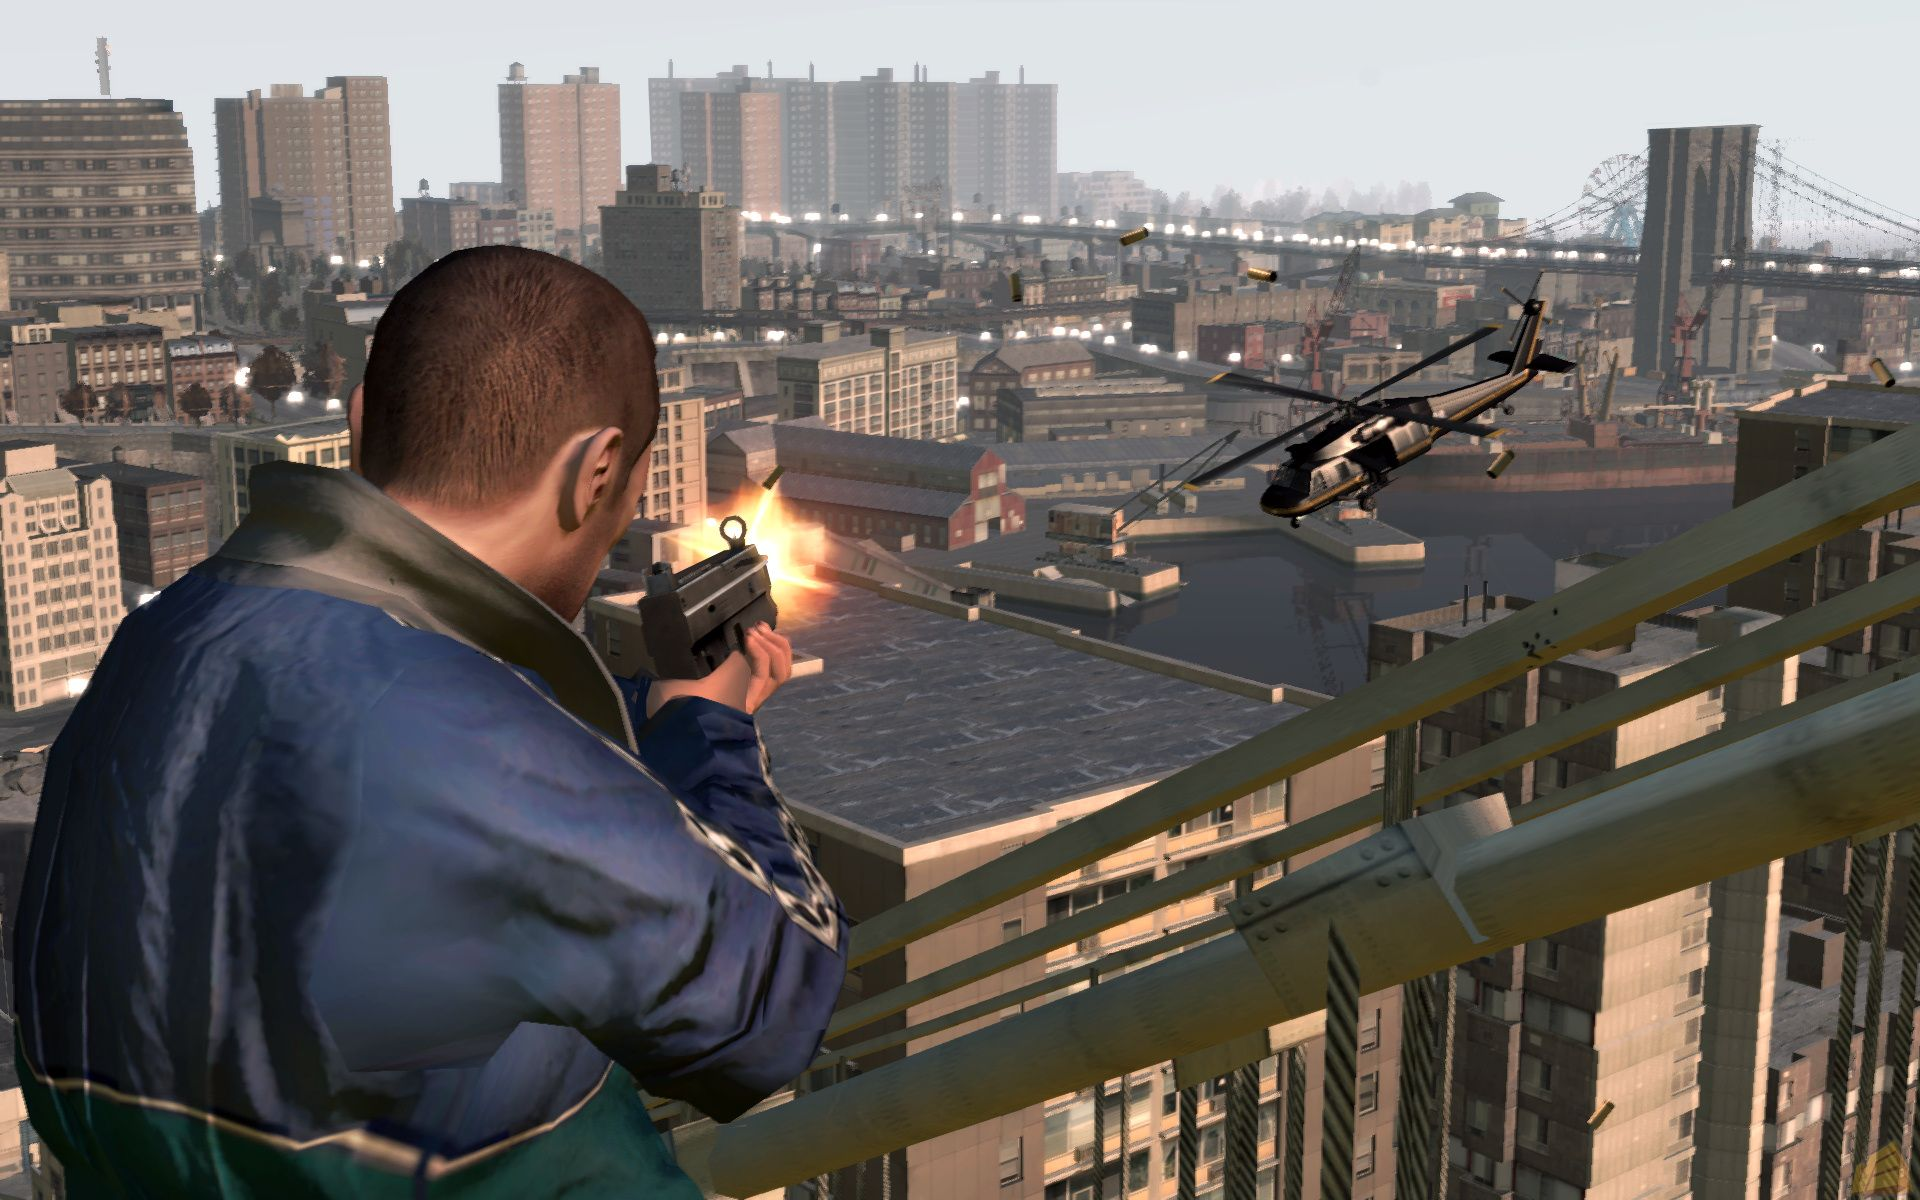
\includegraphics[width=7cm]{GTA4.jpg}
    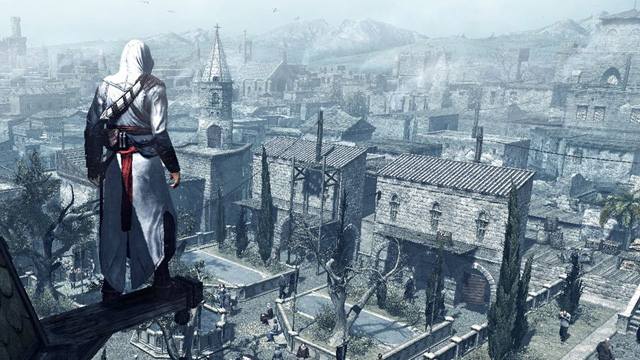
\includegraphics[width=7cm]{AC.jpg}
    \label{villeEx}
\end{figure}

Puisqu'on am�liore le r�alisme de l'environnement autour des personnages, il faut ajouter plus d'information aux formes de la sc�ne. De plus, l'environnement doit toujours �tre plus grand pour donner un meilleur sentiment d'immersion. Il y a un probl�me en ce sens puisque plus il faut d'information pour sp�cifier les formes dans une sc�ne, plus il faut de temps aux artistes pour cr�er cette information. Aussi, cr�er des environnements toujours plus grands demande aussi beaucoup de temps. � un certain point, ce n'est plus envisageable de demander � des gens de faire ce travail. Il faut donc trouver une fa�on d'utiliser la technologie de fa�on intelligente pour faire ce travail automatiquement ou semi-automatiquement. Si on regarde la figure~\ref{villeEx}, on voit qu'il y a beaucoup trop de d�tails dans l'environnement pour que quelqu'un ou une �quipe sp�cifie la position de tous les points de ce mod�le. Ce jeu se d�roule dans un environnement urbain c'est pourquoi l'�tude se poursuit pour cr�er des mod�les d'un environnement urbain. Pour obtenir un bon r�sultat, il est important d'avoir un bon sentiment d'immersion. Pour cela, il faut un bon r�alisme ainsi qu'une bonne vari�t� dans les b�timents de la ville. Par exemple, les images des jeux "Assassin's Creed" et "GTA IV" sont des bons exemples d'environnements r�ussis. La question ici est, comment utiliser la technologie pour arriver a de bons r�sultats de fa�on automatis�e?
